\documentclass[11pt]{article}

\usepackage[utf8]{inputenc}
\usepackage[margin=0.8in]{geometry}
\usepackage{graphicx}
\graphicspath{{data/}}
\usepackage{float}
\usepackage{amsmath}
\usepackage{amssymb}
\usepackage{setspace}
\usepackage{enumitem}
\usepackage{titlesec}
\usepackage{siunitx}
\usepackage{comment}
\usepackage{caption}
\usepackage[version=4]{mhchem}
\usepackage[hidelinks]{hyperref}

\newenvironment{tight_enumerate}{
    \begin{enumerate}[label=(\alph*)]
    \setlength{\itemsep}{3pt}
    \setlength{\parskip}{0pt}}
    {\end{enumerate}}
\DeclareSIUnit{\msun}{
    \text{$M_{\odot}$}
}
\DeclareSIUnit\Angstrom{\AA}
\DeclareSIUnit\year{yr}

\titleformat*{\section}{\large\bfseries}
\titleformat*{\subsection}{\normalsize\bfseries}

\title{\vspace{-2.5em} \textbf{Homework 6}}
\author{Justin Kang \\ AST 381: Star Formation}
\date{\vspace{-0.75em} December 14, 2018}

\begin{document}
\maketitle
\singlespacing
\pagenumbering{gobble}
\sloppy


\vspace{-2.5em}
\section*{Problem 1. Waiting for the dust to settle...}
In this problem we will consider the timescales for dust settling and spatial distribution for different sized silicate dust grains.
\begin{tight_enumerate}
\item Consider particles with $s = 0.1$ and $10$ \si{\micro\meter} located at $r = 1$ \si{AU} in a MMSN disk, where $z = h$, the disk scale height. Assume the disk has a radius of $40$ \si{AU} and the star mass is $M_{*} = 1$ \si{\msun}. Estimate the Reynolds number and determine whether Epstein or Stokes drag applies for each particle size.

\item Find an expression for the terminal velocity of small dust grains with radius $s$ as a function of position $z$ in the disk. Estimate this velocity for the $0.1$ and $10$ \si{\micro\meter} particles described above.

\item Assuming a vertically isothermal disk, show that the settling time can be expressed as 
\[t_\text{settle} = \frac{2\Sigma}{\pi\rho_{m}s\Omega}e^{-z^{2}/2h^{2}},\]
where $\Sigma$ is the disk surface density and $\rho_m$ is the dust density. Compute the settling time for $0.1$ and $10$ \si{\micro\meter} dust grains at $z = h$ and compare these values to other relevant timescales.

\item Now let's consider a turbulent (alpha) disk. Derive an expression for the minimum value of $\alpha$ required to prohibit settling on a scale of $z = h$. Calculate the value of $\alpha$ for $s = 0.1$ and $10$ \si{\micro\meter}. If $\alpha = 10^{-2}$ for an accreting protoplanetary disk, for what grain sizes is settling efficient? Discuss the implications of this result.

\item Consider the dust particles as a separate fluid with density $\rho_{d}$, suspended in a disk with density $\rho$ and subject to the competing influence of settling and turbulent diffusion. Assuming the dimensionless friction time $\Omega{t_\text{fric}}$ is independent of $z$, show that their steady-state density distribution can be described by 
\[\frac{\rho_d}{\rho} = \left(\frac{\rho_d}{\rho}\right)_{0}e^{-z^{2}/2h_d^2},\]
where $h_d$ is the dust scale height, 
\[h_d = \sqrt{\frac{\alpha{c_s^2}\rho{c_s}}{\Omega^{3}\rho_{m}s}}.\]
\end{tight_enumerate}

\subsection*{Solution 1}
\begin{tight_enumerate}
\item The Reynolds number is defined as $\text{Re} = \frac{sv}{{\lambda}c_s}$, where $s$ is the grain size, $v$ the grain velocity, $\lambda$ the mean free path, and $c_s$ the sound speed. The mean free path is given by $\lambda = \frac{1}{n\sigma} = \frac{{\mu}m_{\ce{H}}}{{\rho_0}\sigma}$, where $\mu = 2.3$ on average for interstellar material and $\rho_0$ is the disk midplane density. To solve for the midplane density, we solve the hydrostatic equilibrium equation:
\[\frac{\partial P}{\partial z} + \rho g_z = 0 \implies \frac{1}{\rho}\frac{\partial P}{\partial z} = -g_z.\]
Assuming vertical isothermality, 
\[P = \rho c_s^2,\]
and we know that for a point at height $z$ and distance $r$ away from the star on the disk, 
\[g_z = g\sin\theta \approx \frac{GM_*}{r^2}\sin\theta \approx \frac{G M_* z}{r^3} = \Omega^2 z.\]
Plugging these in, we find that 
\[\frac{\partial \ln\rho}{\partial z} = -\frac{\Omega^2}{c_s^2}z = -\frac{z}{h^2},\]
where $h = \frac{c_s}{\Omega}$ is the disk scale height. Solving, we find that 
\[\ln\rho = \ln\rho_0 - \frac{z^2}{2h^2} \implies \rho(z) = \rho_0 e^{-z^2/2h^2}.\]
We can relate this to the disk surface density by 
\[\Sigma = \int_{-\infty}^{\infty} \rho(z)dz = \sqrt{2}h\rho_0\int_{-\infty}^{\infty}e^{-x^2}dx = \sqrt{2\pi}h\rho_0,\]
giving us 
\[\rho_0 = \frac{\Sigma}{\sqrt{2\pi}h}.\]
Setting $z = h$, $\Sigma \approx (1700\ \si{\gram\per\square\centi\meter})\left(\frac{r}{\si{AU}}\right)^{-3/2}$, and taking the MMSN relation $h \approx 0.03\left(\frac{r}{\si{AU}}\right)^{5/4}$ \si{AU}, we find that 
\[\rho(z=h) = \frac{1700\ \si{\gram\per\square\centi\meter}}{\sqrt{2\pi}(0.03\ \si{AU})}e^{-1/2} \approx 10^{-9}\ \si{\gram\per\cubic\centi\meter}.\]
Setting the cross-sectional area of the hydrogen to be ${\sim}2$ \si{\Angstrom}, the mean free path is then 
\[\lambda \approx \frac{2.3m_{\ce{H}}}{(10^{-9}\ \si{\gram\per\cubic\centi\meter})(2\ \si{\Angstrom})^2} \approx 10\ \si{\centi\meter}.\]
We note that the mean free path is much longer than either of the grain sizes.\\
\fbox{$\therefore$ Epstein drag will apply for both particle sizes.}\\
Assuming an ideal gas, we can expand the definition of the Reynolds number to be 
\[\text{Re} = \frac{sv}{\lambda c_s} = \frac{s\sqrt{GM_*/r}}{\lambda\sqrt{kT/m}}.\]
To find the temperature at $(r,z)$, we know that 
\[F_* \equiv \frac{L_*}{4\pi r^2}.\] 
Setting the input power of the dust at $(r,z)$ equal to the output power of the dust, we have 
\[\pi s^2 F_* = 4\pi s^2 \sigma_{SB}T^4 \implies T = \left(\frac{F_*}{4\sigma_{SB}}\right)^{1/4} \approx 278.33\ \si{K},\]
assuming that the star has solar luminosity. Plugging all of these in, we can finally obtain our Reynolds numbers.\\
\fbox{$\therefore$ $\text{Re}(s=0.1\ \si{\micro\meter}) \approx 2 \cdot 10^{-5}$, $\text{Re}(s=10\ \si{\micro\meter}) \approx 0.002$.}

\newpage
\item The equation for Epstein drag is given by 
\[F_D = \frac{4\pi}{3}s^2\rho v v_{th},\]
where $v_{th} = \sqrt{\frac{8kT}{\pi m}}$ is the thermal velocity. 
where $\rho_m$ is the dust density. We know that for settling, gravity and drag will be the two forces at play. Given our earlier expression for $g_z = \Omega^2 z$, we can thus equate forces to find 
\[m\Omega^2 z = \frac{4\pi}{3}s^2 \rho v v_{th}.\]
We can then solve for $v$ to obtain the terminal velocity.\\
\fbox{$\therefore$ $v(s,z) = \frac{3m\Omega^2 z}{4\pi s^2 \rho v_{th}}$.}\\
The dust density for a MMSN is approximately $\rho_m \approx 3$ \si{\gram\per\cubic\centi\meter}, so we can then plug in our two grain sizes to obtain the numerical terminal velocities for the grains.\\
\fbox{$\therefore$ $v(s=0.1\ \si{\micro\meter},z=h) = 2.760*10^{-6}$ \si{\meter\per\second}, $v(s=10\ \si{\micro\meter},z=h) = 2.760*10^{-4}$ \si{\meter\per\second}.}

\item Defining the "stopping time" as $t_s = \frac{mv}{F_D}$, we can substitute the form of Epstein drag to obtain 
\[t_s = \frac{mv}{\frac{4\pi}{3}s^2 \rho v v_{th}} = \frac{m}{\frac{4\pi}{3}\pi s^3}\frac{s}{\rho v_{th}} = \frac{\rho_m s}{\rho v_{th}}.\]
The settling time is defined as $t_z = \frac{z}{v}$. Setting $v$ as our terminal velocity obtained in (b), 
\[t_\text{settle} = \frac{\frac{4\pi}{3}s^3}{m}\frac{\rho v_{th}}{s}\frac{1}{\Omega^2} = \frac{1}{t_s}\frac{1}{\Omega^2} = \frac{\rho v_{th}}{\rho_m s}\frac{1}{\Omega^2}.\]
Inputting our $\rho(z)$ from (a),
\[t_\text{settle} = \frac{v_{th}}{\rho_m s}\frac{1}{\Omega^2}\frac{\Sigma}{\sqrt{2\pi}h}e^{-z^2/2h^2} = \frac{\Sigma}{\rho_m s}\frac{1}{\Omega}\frac{1}{\sqrt{2\pi}}\frac{v_th}{c_s}e^{-z^2/2h^2}.\]
For an ideal gas $c_s = \sqrt{\frac{kT}{m}}$, so 
\[t_\text{settle} = \frac{\Sigma}{\rho_m s}\frac{1}{\Omega}\frac{1}{\sqrt{2\pi}}\sqrt{\frac{8}{\pi}}e^{-z^2/2h^2} = \frac{2\Sigma}{\pi \rho_m s\Omega}e^{-z^2/2h^2}.\]
\fbox{$\therefore$ $t_\text{settle} = \frac{2\Sigma}{\pi \rho_m s\Omega}e^{-z^2/2h^2}$.}\\
\fbox{$\therefore$ $t_\text{settle}(s=0.1\ \si{\micro\meter}) \approx 3.48\cdot10^6$ \si{\year}, $t_\text{settle}(s=10\ \si{\micro\meter}) \approx 3.48\cdot10^4$ \si{\year}.}\\
Considering how we expect a disk lifetime to be around $10$ \si{\mega\year}, we find these answers to be reasonable as the dust needs to settle within the disk lifetime in order to produce planets.

\item In order to prohibit settling, we require that the diffusion timescale be shorter than the settling timescale. This then gives us the relation 
\[t_\text{diff} \approx \frac{z^2}{\nu} = \frac{z^2}{\alpha c_s h} \leq t_\text{settle},\]
where $\nu = \alpha c_s h$ under the alpha disk treatment. Writing in the full form of the settling time and using $h = \frac{c_s}{\Omega}$, 
\[\frac{z^2}{\alpha h^2\Omega} \leq \frac{2\Sigma}{\pi \rho_m s\Omega}e^{-z^2/2h^2}.\]
Setting $z = h$, 
\[\frac{h^2}{h^2}\frac{1}{\alpha\Omega} \leq \frac{2\Sigma e^{-1/2}}{\pi \rho_m s\Omega},\]
from which we can then solve for the minimum $\alpha$.\\
\fbox{$\therefore$ $\alpha = \frac{\pi\rho_m s e^{1/2}}{2\Sigma}$.}\\
\fbox{$\therefore$ $\alpha(s=0.1\ \si{\micro\meter}) = 4.57\cdot10^{-8}$, $\alpha(s=10\ \si{\micro\meter}) = 4.57\cdot10^{-6}$.}\\
Assuming that $\alpha = 10^{-2}$, we find that $s \approx 2.2$ \si{\centi\meter}. Knowing that dust must eventually settle into the midplane to form planets, this implies that particle sizes must be greater than an order of a centimeter in order to properly settle for a protoplanetary disk.

\item Since we consider the dust as a separate fluid suspended in the disk, we can treat dust settling as convection (settling is the bulk motion of the dust). Using the convection-diffusion equation, we can then compare the settling and turbulent diffusion to obtain the steady-state density distribution. Since we only care about the $z$-component of the motion, the diffusion component has the form 
\[\frac{\partial \rho_d}{\partial t} = \frac{\alpha c_s^2}{\Omega}\frac{\partial}{\partial z}\left[\rho\frac{\partial}{\partial z}\left(\frac{\rho_d}{\rho}\right)\right],\]
and the convection component has the form 
\[\frac{\partial \rho_d}{\partial t} = -\frac{\partial}{\partial z}(\Omega^2 t_\text{fric}\rho_d z),\]
where $t_\text{fric} \equiv \frac{\rho_d}{\rho}\frac{s}{c_s}$. We can add the effects of both to form a continuity equation, and under the steady state assumption we know that $\frac{\partial \rho_d}{\partial t} = 0$. Thus 
\begin{align*}
\frac{\alpha c_s^2}{\Omega}\frac{\partial}{\partial z}\left[\rho\frac{\partial}{\partial z}\left(\frac{\rho_d}{\rho}\right)\right] &= -\frac{\partial}{\partial z}(\Omega^2 t_\text{fric}\rho_d z),\\
\frac{\alpha c_s^2}{\Omega}\int\frac{\partial}{\partial z}\left[\rho\frac{\partial}{\partial z}\left(\frac{\rho_d}{\rho}\right)\right] &= -\Omega^2 t_\text{fric}\rho_d\int1,\\
\frac{\alpha c_s^2}{\Omega}\left[\rho\frac{\partial}{\partial z}\left(\frac{\rho_d}{\rho}\right)\right] &= -\Omega^2 t_\text{fric}\rho_d z,\\
\frac{\rho}{\rho_d}\frac{\partial}{\partial z}\left(\frac{\rho_d}{\rho}\right) &= -\frac{\Omega^3 t_{\text{fric}}}{\alpha c_s^2} z,\\
\int\frac{\partial}{\partial z}\ln\left(\frac{\rho_d}{\rho}\right) &= -\frac{\Omega^3 t_{\text{fric}}}{\alpha c_s^2}\int
z,\\
\ln\left(\frac{\rho_d}{\rho}\right) &= \left(\frac{\rho_d}{\rho}\right)_0 - \frac{\Omega^3 t_{\text{fric}}}{\alpha c_s^2} z^2 = \left(\frac{\rho_d}{\rho}\right)_0 - \frac{\Omega^3 \rho_d s}{\alpha c_s^2 \rho c_s} z^2,\\
\frac{\rho_d}{\rho} &= \left(\frac{\rho_d}{\rho}\right)_0 e^{-z^2/2h_d^2},
\end{align*}
where $h_d \equiv \sqrt{\frac{\alpha c_s^2 \rho c_s}{\Omega^3 \rho_m s}}$ is the dust scale height.\\
\fbox{$\therefore$ $\frac{\rho_d}{\rho} = \left(\frac{\rho_d}{\rho}\right)_{0}e^{-z^{2}/2h_d^2}$.}
\end{tight_enumerate}



\newpage
\section*{Problem 2. Cooking up complex chemistry.}
In this problem you will model the astrochemistry of a protoplanetary disk using the Nahoon gas-grain astrochemistry code. You can download the latest version here: \url{http://kida.obs.u-bordeaux1.fr/codes.html}. Use the KIDA 2014 reaction network that is contained in the download. Note, the package includes IDL routines for reading and plotting the abundances; you can use these or create your own version in Python.

\begin{tight_enumerate}
\item Modify the input parameter file to model gas with $\rho = 2\times10^{10}$ \si{\gram\per\cubic\centi\meter}, $T = 10$ \si{\kelvin}, CRIR = $1.3\times10^{-17}$ \si{\per\second}, $s = 10^{-5}$ \si{\centi\meter} silicate grains. Produce plots of the abundance ratios \ce{HC3N}/\ce{HCN} and \ce{CH3CN}/\ce{HCN} as functions of time. Explain any trends with time. Do your results agree with those of Oberg et al. (2015)? Why or why not?

\item Vary the gas temperature and dust size separately over several orders of magnitude. What impact does this variation have on the \ce{HCN}, \ce{HC3N}, and \ce{CH3CN} abundances and the abundance ratios in (a)? Does this agree with your expectations and why?

\item The CRIR may be a couple orders of magnitude lower than the "fiducial" Galactic value in the disk midplane due to attenuation (e.g., Cleeves et al. 2014). Meanwhile the CRIR may be an order of magnitude higher at the disk surface due to CR accelerated in accretion shocks (Gaches \& Offner 2018b). Vary this parameter over several orders of magnitude. What effects does this have on the abundances and level of agreement with the ratios reported by Oberg et al.?

\item Pick another species included in the chemical network that you think is interesting or important for understanding protoplanetary disks. Explore its abundance over a range of different physical conditions. Justify your choice of species (why should it be interesting) and report the result of your numerical experiments (e.g., for what times and parameters is the abundance the highest, lowest, etc.).
\end{tight_enumerate}

\subsection*{Solution 2}
\begin{tight_enumerate}
\item The abundance ratios \ce{HC3N}/\ce{HCN} and \ce{CH3CN}/\ce{HCN} are shown in Figure 1. In both cases we see a similar trend: the abundances rise until around $t {\sim} 10^5$ years, drop off significantly, rise again until $t {\sim} 10^6$ years, then drop and level off. The initial rise can likely be explained by the gradual formation of the reactants needed to produce these species. A reason for the drop may be explained by other species using up the reactants, as well as these species being used as the reactants for other products. Eventually the abundances reach their steady state values and level off.\\
\indent Oberg et al. (2015) estimate that \ce{HC3N}/\ce{HCN} and \ce{CH3CN}/\ce{HCN} at $30$ \si{AU} are $0.$ and $0.05$, and $5$ and $0.2$ at $100$ \si{AU}. The authors admit these are overestimates, and give more conservative estimates of $5\%$ and $20\%$ at $30$ and $100$ \si{AU}. Looking at $t {\sim} 10^6$ years, the estimated age of MWC 480, we find that there is reasonable agreement with the $30$ estimate for \ce{HC3N}/\ce{HCN}, but that our estimates are orders of magnitude less than their estimates for \ce{CH3CN}/\ce{HCN}. This could possibly be due to the other input factors, such as the grain size, gas density, or gas temperature, that went into the model. 
\begin{figure}[H]
\centering
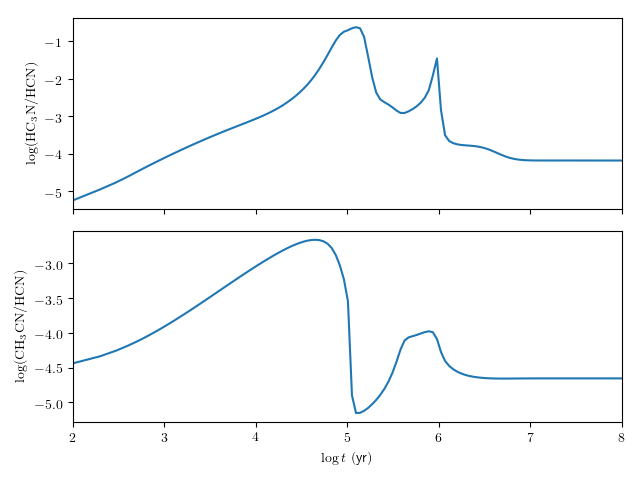
\includegraphics[height=0.45\textheight]{a/ratios.png}
\caption{The abundance ratios \ce{HC3N}/\ce{HCN} and \ce{CH3CN}/\ce{HCN} as functions of time.}
\end{figure}

\item The abundances as functions of time and gas temperature, and time and grain size are shown in Figure 2. The abundance ratios as functions of time and temperature, and time and grain size are shown in Figure 3. When we vary the temperatures, we find that for $10^{-1}{-}10^1$ \si{K}, the behavior of the particles is mostly the same, with the abundances being offset such that at higher temperatures the trends occur sooner. This is reasonable, because at lower temperatures it will take a longer time for these more complex molecules to start forming. However, we see significant changes as the temperature increases. Surpisingly at $10^2$ \si{K} we see a dropoff in the abundances of the molecules, and then at $10^3$ \si{K} we see the abundances increase by many orders of magnitude. This could be a numerical artifact, as it doesn't make too much sense that the abundances would go down than significantly up. One explanation for this is that at those high temperatures the reaction rates for these molecules go so far up that there are orders of magnitude more in abundance of these particles. The ratios are quite different, however. For both cases, we again see similarity between the $10^{-1}{-}10^1$ \si{K} ratios and our results from (a). For \ce{HC3N}/\ce{HCN} we still observe the weird behavior early on for $10^2{-}10^3$ \si{K}, they approach similar steady state values after around a Myr. However for \ce{CH3CN}/\ce{HCN}, although the $10^2$ \si{K} behavior is very simliar to the rest, the $10^3$ \si{K} jumps orders of magnitude above the rest for steady state value, agreeing with the expectations from the abundances.\\
\indent\hspace{1em} In terms of grain sizes, we find that there is little variation in both the abundances and abundance ratios for $10^{-7}\ \si{\centi\meter} \leq s \leq 10^{-3}\ \si{\centi\meter}$, suggesting that the reaction rates (and thus production) of these particles are not limited by grain sizes. This is a little surprising as dust surface chemistry is important. There is some variation at the largest scale ($10^{-3}$ \si{\centi\meter}), suggesting that any other size within the input range is good enough to facilitate the formation of these molecules.
\begin{figure}[H]
\centering
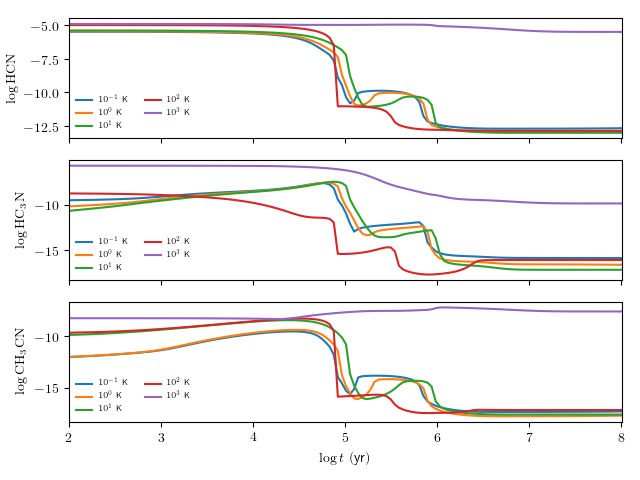
\includegraphics[height=0.45\textheight]{b/t_abundances.png}
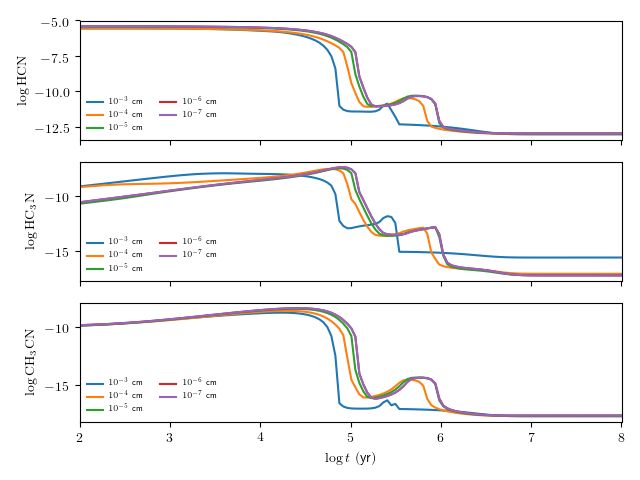
\includegraphics[height=0.45\textheight]{b/s_abundances.png}
\caption{The abundances of the selected species as functions of time and gas temperature.}
\end{figure}
\begin{figure}[H]
\centering
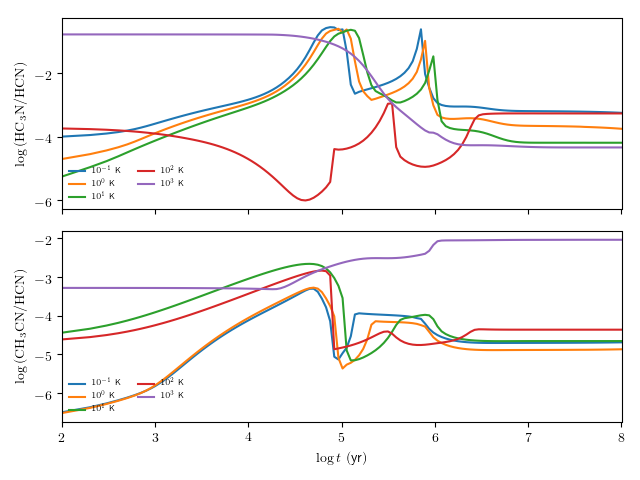
\includegraphics[height=0.45\textheight]{b/t_ratios.png}
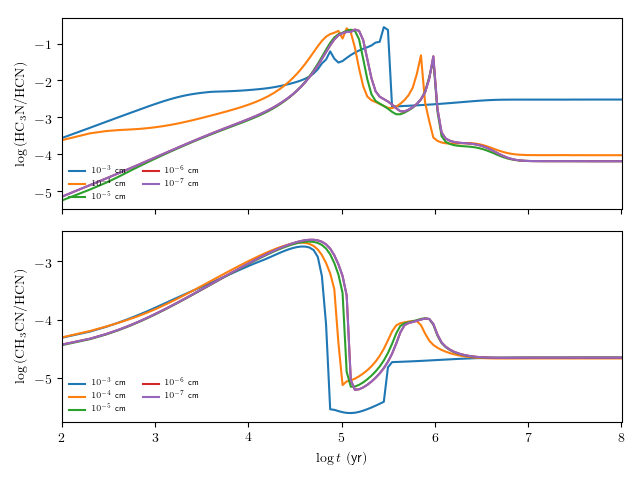
\includegraphics[height=0.45\textheight]{b/s_ratios.png}
\caption{The abundance ratios of the selected species as functions of time and dust size.}
\end{figure}

\newpage
\item As we vary the cosmic ray ionization rate, we find that the general behavior remains the same, just that things happen earlier as you increase the ionization rate. This conceptually makes sense as although CRIR does destroy some particles, it can also provide heat to the disk for endothermic reactions and set off reactions. Thus increasing the CRIR basically accelerates the rates at which the processes affecting the abundances of the species occurs, which is reasonable. The trend from (a) continues in terms of agreement with Oberg et al.: at amount a megayear the \ce{HC3N}/\ce{HCN} ratio relatively agrees with the $30$ \si{AU} estimate, but the \ce{CH3CN}/\ce{HCN} ratio is orders of magnitude below all estimates. However, the authors note that in their own testing none of their own models could produce $\ce{CH3CN}/\ce{HCN} > 0.01$ and that the vast majority of the parameter space lied in $\ce{CH3CN}/\ce{HCN} < 0.001$, which agrees with our results. 

\begin{figure}[H]
\centering
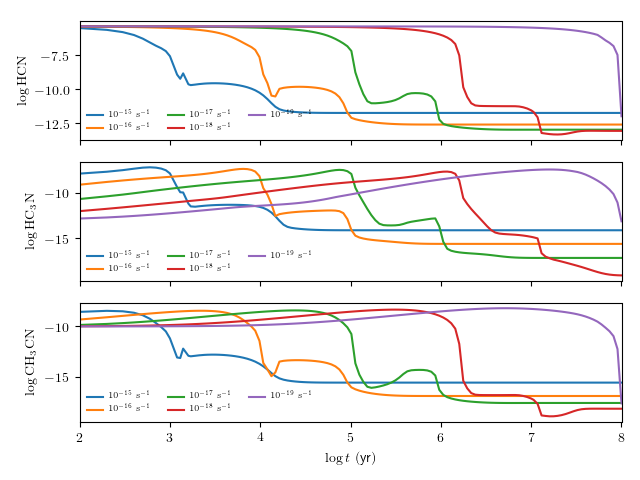
\includegraphics[height=0.45\textheight]{c/abundances.png}
\caption{The abundances of the selected species as functions of time and CRIR.}
\end{figure}
\begin{figure}[H]
\centering
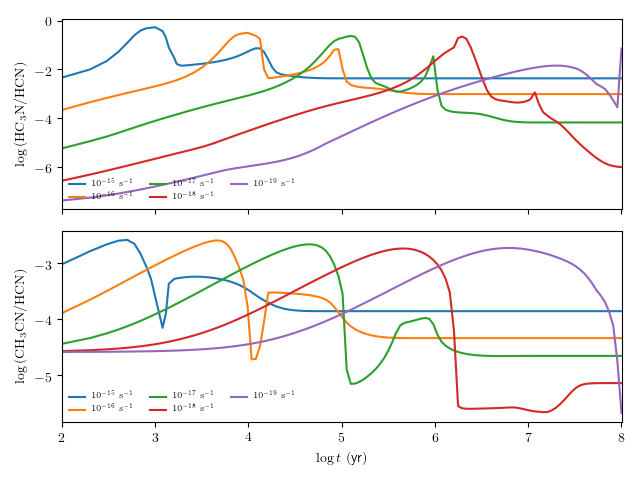
\includegraphics[height=0.45\textheight]{c/ratios.png}
\caption{The abundance ratios of the selected species as functions of time and CRIR.}
\end{figure}

\item For our own experiment we vary the gas temperature and grain size (the same as in (b)) and measure its effects on the abundance of \ce{H2O}. \ce{H2O} is obviously an important molecule because it is the essential molecule for life, and tracing its abundance during the protoplanetary disk stage can help us understand what initial conditions can lead to life (or habitable planets). In both cases, we see similar behavior to what we found for the cyanides in (b). As we vary the temperature, the overall behavior for the $10^{-1}{-}10^2$ \si{K} range is similar. These start off at nearly the same initial conditions, but after around ${\sim}10^5$ years, they divergence and end up with about an order of magnitude difference in their steady state values. We again observe that for $T = 10^3$ \si{K}, the abundance is orders of magnitude higher than the rest and relatively flat. This again might be due to a numerical artifact, as having a $1000$ \si{K} disk while keeping all other values relatively "normal" seems unphysical. Ultimately, this shows us that the abundance of water is decently sensitive to changes in temperature, which could be important.\\
\indent\hspace{1em} In terms of grain size, basically all of the sizes excluding the two largest sizes follow the exact same curve. The second largest size ($10^{-4}$ \si{\centi\meter}) has slightly lower steady state values, whereas the largest size ($10^{-3}$ \si{\centi\meter}) has a significantly lower value throughout the run. Considering how formation mechanisms of \ce{H2O} generally involve \ce{H2}, this is not surprising. If the grain size is too large then the reaction to form \ce{H2} will take long due to the large amount of hopping or luck needed, and this decreased abundance in \ce{H2} will naturally lead to a decrease in \ce{H2O}. Ultimately this lets us know that as long as the grains aren't too large, water will form pretty regularly in protoplanetary disks.

\begin{figure}[H]
\centering
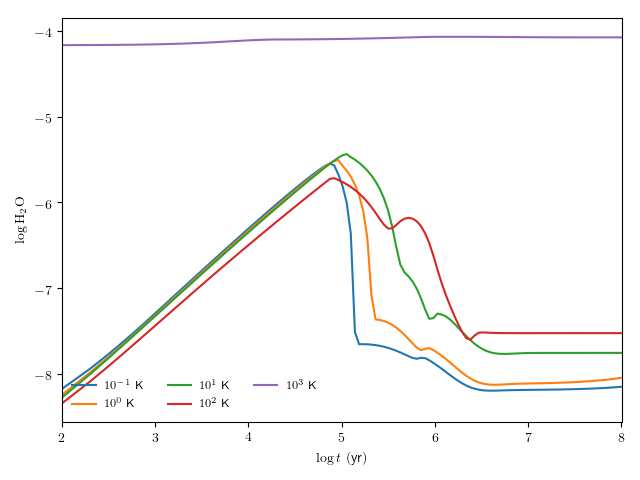
\includegraphics[height=0.45\textheight]{d/t_abundances.png}
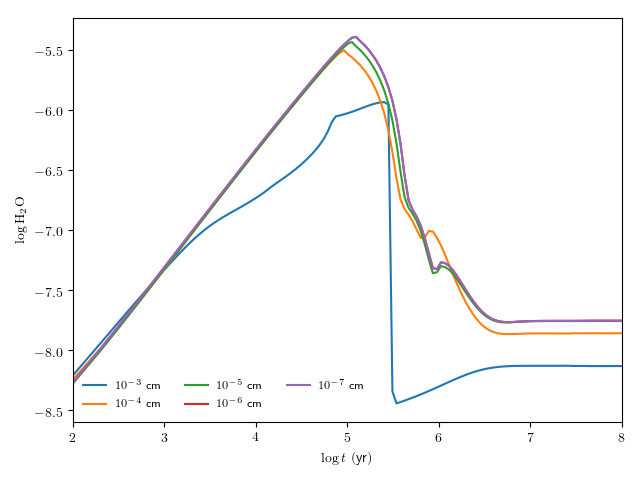
\includegraphics[height=0.45\textheight]{d/s_abundances.png}
\caption{The abundance of \ce{H2O} as functions of time and gas temperature, and time and dust size.}
\end{figure}
\end{tight_enumerate}


\end{document}